\chapter{Human simulated functional testing (HSUF)}

Human simulated functional testing (HSUF) consists of use of camera to detect icons or perform optical character recognition (OCR) and then use
robot to perform movements according to detection results. A typical use case is to find an icon on DUT screen with camera and then perform tap gesture on detected location of the icon.

\importantbox{If you are using HSUF via TnT Client, make sure that the camera is not open in TnT UI. Having the camera open in more than one instance might interfere with Client script execution.}

\section{Screenshots}

When user performs OCR or icon detection via TnT Client, the robot will move the camera over the designated DUT so that the DUT center appears at the center of the camera and the DUT surface is at the focal point of the camera. In case the DUT is rotated with respect to the camera view, the image is automatically rotated in software and cropped so that the DUT appears upright. This image is referred to as the \emph{screenshot}. See Figure \ref{fig:screenshot} for illustration.

\begin{figure}[h]
	\centering
	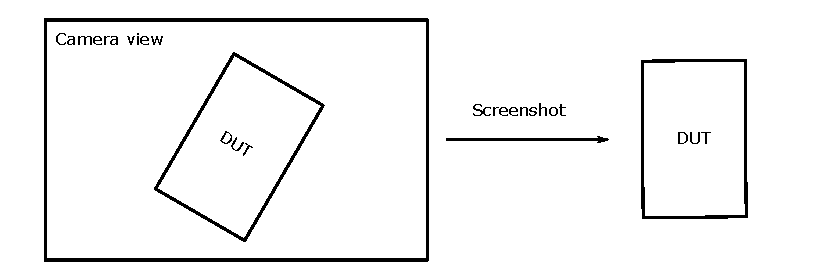
\includegraphics[width=\linewidth]{screenshot.pdf}
	\caption{Taking a screenshot of DUT with camera.}
	\label{fig:screenshot}
\end{figure}

In usual robot systems the positioning camera is attached to the z-axis of the robot and cannot rotate. Nevertheless DUTs in the workspace don't have to be aligned in any specific way in order to do functional testing due to aforementioned image transformation. 

OCR and icon detection is then applied on the screenshot image. See the docstring \texttt{TnTDutClient} \texttt{.screenshot()} for detailed description of the available parameters.

Note that the DUT must fit within the camera view in order to effectively perform functional testing. The system does not automatically try to scan over large DUT to find objects although it is possible for user to implement such behaviour by using specific offset parameters in TnT Client. In typical configuration where the camera is fixed to the robot z-axis, the robot must move between each detection and gesture which takes some amount of time. If the robot has a rotating tool, it is automatically rotated away from the camera view when taking a screenshot.

User can use TnT Client to take a screenshot of a DUT. The image is stored in TnT Server and can then be accessed via the client to perform additional tasks. User can perform OCR and icon detection on the image, do image manipulation such as cropping and color inversion or implement custom detection algorithms. Note that usually cameras have a limited capture frequency depending on resolution, connection interface and cost. Often the frame rate is as low as 5 frames per second so implementing e.g. blink detection might not be possible even though the API makes it possible in theory. Some cameras support hardware binning which can be used to downscale the camera image and hence improve the frame rate.

\section{Optical character recognition}
TnT Server implements OCR by relying on third-party libraries. These are implemented as \emph{drivers} so that user
can select appropriate OCR driver for specific use cases. Some drivers perform better that others in different use cases.
Currently following drivers are supported:
%
\begin{itemize}
\item ABBYY
\item Tesseract
\end{itemize}

ABBYY requires a commercial license, which is included in functional tester (HSUF) deliveries by default, unless agreed otherwise. Tesseract uses an open source license.

OCR can only be used via TnT Client API to create user specific test scripts. There are two APIs for finding text: \texttt{TnTDUTClient.search{\_}text()} and \texttt{TnTImageClient.search{\_}text()}. The first API method takes a screenshot as described above, saves the image file and perform OCR on the image. The OCR results i.e. the detected locations of text objects are returned in mm units in DUT context. These results can then be directly used in gesture API to perform e.g. a tap gesture on the detected location. The latter API method can be used on an existing image resource to find text on the image.

All provided OCR drivers are sensitive to defects in the image. These defects are basically anything other than text including
noise, reflections from the screen, background images, moire etc. The drivers tend to perform poorly without any filtering.
For example Tesseract is designed to find dark text on light background. If the opposite is true for the target image, user should invert the colors before performing OCR. In order to apply filtering, the \texttt{TnTDUTClient.search{\_}text()} has filter parameter that
can be used to specify an existing image filter script before OCR is performed. With \texttt{TnTImageClient.search{\_}text()}, user can
first call \texttt{TnTImageClient.filter()}. This is what also \texttt{TnTDUTClient.search{\_}text()} calls under the hood if filter parameter is given.

The filters are Python files located under \texttt{data/image{\_}filters} directory under TnT Server installation. The filter parameter
of \texttt{TnTDUTClient.search{\_}text()} is the name of a file in that directory without extension ".py". For example:

\begin{lstlisting}[language=Python]
dut = TnTDUTClient("mydut")
results = dut.search_text("Hello world!", filter="ocr")
\end{lstlisting}

The rationale that filters are stored under such location is as follows: \texttt{data} is considered to be customer specific. If
a new version of TnT Server is installed, the data directory is always retained from previous installation. The image processing
scripts may change in future revisions as we discover better ways to improve filtering for OCR. However, any changes may
break existing customer test cases as they might perform worse in specific scenarios. This approach by default retains compatibility.

When performing OCR, following things should be considered:

\begin{itemize}
\item There should be no significant reflections from the DUT visible in the camera image over the text to be detected. Even changes in background gradient due to reflections can affect the results.
\item The camera exposure and gain should be adjusted so that the text is not over nor under exposed.
\item If possible, the image should be cropped so that there is not much additional content in the image. Especially ABBYY gets confused by additional graphics and might not find anything until the image is cropped around the text.
\item Tesseract is designed to find dark text over white background. Invert image colors if this is not true for the original image. Most often in smart device testing the colors need to be inverted.
\item Text should appear upright in the screenshot image. Rotated text is usually not detected.
\item ABBYY does not give a score for the detected results. If no text pattern is provided for OCR, the score will be 1.0 for all found results. If pattern is given, it is matched against ABBYY results and a score is computed based on this matching.
\item Both ABBYY and Tesseract can fail to detect text in some circumstances. Sometimes it is necessary for user to write trial-and-error heuristics on top of the provided API to perform well in the user specific test cases.
\item The OCR drivers have certain limits for the size of text in pixels. Tesseract can usually only recognize characters of height 10 px - 30 px. User may need to rescale screenshots if the text size falls out of this range.
\item Background image behind the text may reduce the reliability of OCR.
\end{itemize}

\section{Icon teaching}

Icon teaching is usually done manually by cropping images from camera view using TnT UI. See Section \ref{sec:ui_icon_teaching} for more information.

It is also possible to teach icons from existing image files using Python and TnT Client.

\section{Icon detection}

TnT Server implements icon detection based on third-party Halcon software package. Halcon requires a commercial license, which is included in functional tester (HSUF) deliveries by default, unless agreed otherwise.

The icon detection has actually two distinct parts: 1) Icon teaching and 2) icon detection. 

The first part is done before-hand. An image is converted into a shape model which is then stored and used in the actual icon detection. The parameters used in the shape model generation affect how well the icon will be detected in various circumstances. For example how many different scalings and rotations of the icon can be detected. Currently these parameters are fixed according to our experience on icon detection in smart device functional testing.

The second part consists of taking an image (usually with a camera attached to the robot) and detecting an icon using the existing shape model. The second part can only be performed via Python scripts using TnT Client. See \texttt{TnTDutClient.find\_objects()} and its docstring for the possbile parameters that can be used in icon detection. This method works similar to the OCR counterpart i.e. it takes a screenshot and then detects icon from the resulting image. To detect icons directly from existing image, see \texttt{TnTImageClient.find\_objects()}. See also example scripts under \texttt{tntclient/examples} in the TnT Client Python package.

Icon detection tends to be very sensitive to differences between the image that was used to teach the icon and then the image where the icon is attempted to be found. Following things should be considered:

\begin{itemize}
\item Use the same camera exposure and gain when teaching the icons and when detecting the icons. This is not enforced by default so user must provide \texttt{exposure} and \texttt{gain} parameters to the icon detection API.
\item Teaching icons from ideal reference images is possible via TnT Client but it might not work in detection if the icon appears differently scaled and colored in the camera image during detection.
\item Make sure that the lighting conditions in the test area are the same when teaching icons and when detecting icons.
\item There should be no significant reflections from the DUT visible in the camera image when detecting icons.
\item Icon taught in upright orientation might not be detected with good confidence if it appears rotated in the screenshot.
\item If icon appears on the camera image at different scale than in the taught model, it might not be recognized. Usually icons sizes 1x and 2x of the taught icon are found with good confidence.
\item Cropping screenshot around icon to be detected may also help in case the icon is not detected from the entire image.
\end{itemize}

\subsection{Colored icon detection}

Halcon builds a contour shape model of the icon which does not consider color in any way. By default, icon detection does not take the color into account. However the original icon image is also stored in addition to the shape model and this can be used to take color into account. The idea is that once the icon shape is found with Halcon, a color comparison algorithm is used to weight the Halcon score based on the color similarity. Hence it is possible to distinguish icons that have the same shape but different color.

In order to enable color comparison, TnT Server configuration file must have color comparison method specified:

\begin{lstlisting}[language=Python]
- name: halcon
  cls: TnT.Detector
  parent: detectors
  connection: detectors
  arguments:
    driver: Halcon
    color_cmp_method: template
    color_cmp_params:
      threshold: 0.2
\end{lstlisting}

Comparing the color between two images is not always simple. Therefore there are multiple color comparison methods available. The best one should be selected based on particular use case. Possible methods are \texttt{template}, \texttt{histogram} and \texttt{moments}. For each method certain parameters can be given to adjust the behavior of the algorithm. Each method accepts \texttt{threshold} parameter in range [0, 1] which clamps intensity below threshold to zero. This can be effective to remove colored dark background gradient from biasing the color comparison.
